\begin{center}
    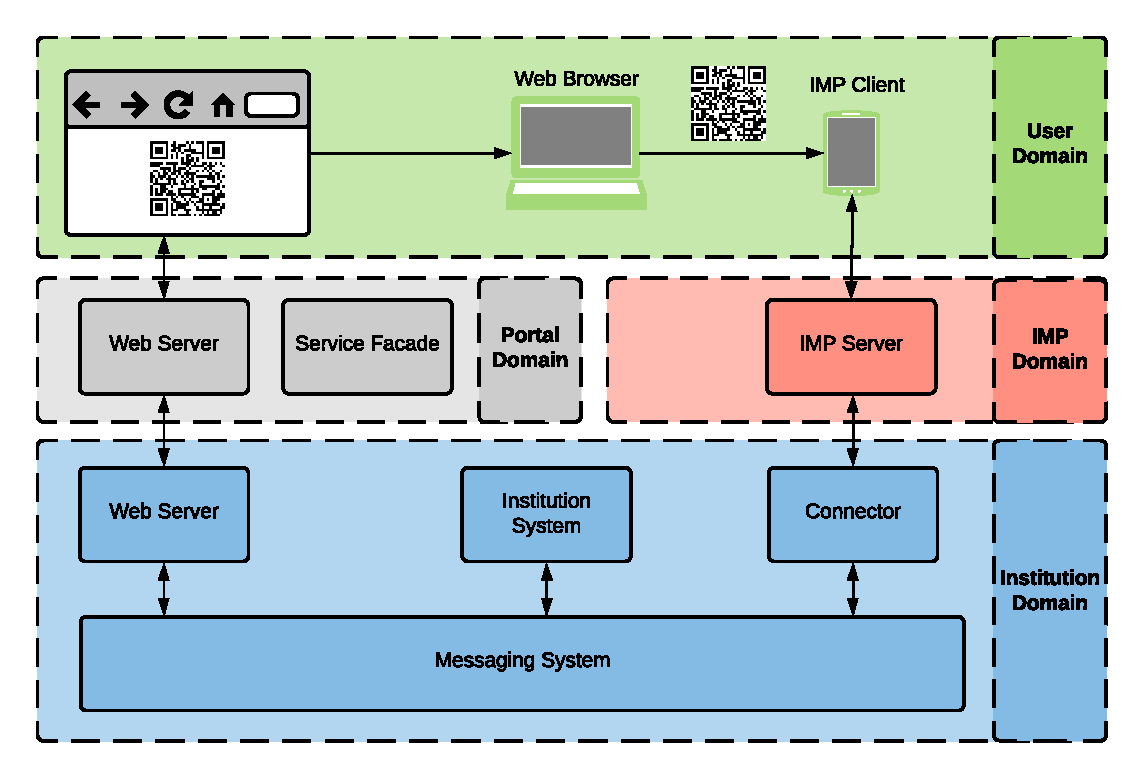
\includegraphics[scale=0.6]{Diagrams/Integration Architecture 2/Overview.pdf}
\end{center}

To implement the solution described in the previous section, a connector is included in the existing system architecture of every institution. The same messaging system described in chapter 4 can be used to integrate the IMP solution described in the previous section. Many of the messaging modules can be reused with minor modifications. Similar to the messaging system in chapter 4, two system components are connected: A web server and a institution system.

As described in the previous section, for each administrative service, the institution is able to process, a relationship template is created and stored on a web page displayed by the web server. This can be done, as no personalized relationship templates will have to be created. 

Therefore, the messaging system wont need modules for creating templates. However, modules for processing incoming relationship requests are required.

\begin{center}
    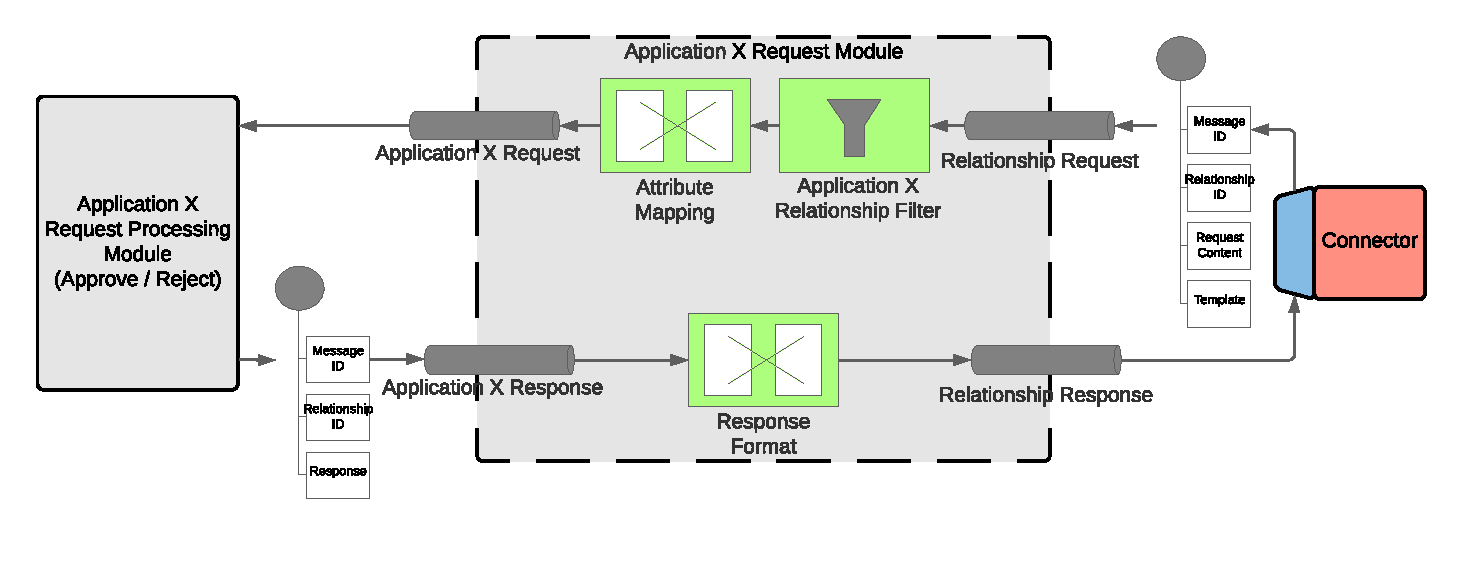
\includegraphics[scale=0.6]{Diagrams/Integration Architecture 2/Application Request Module.pdf}
\end{center}

For each administrative service, separate types of relationship templates and therefore relationship requests exist. Each relationship request type is processed by its custom "Application Request" module and "Application Request Processing" module. 

\begin{center}
    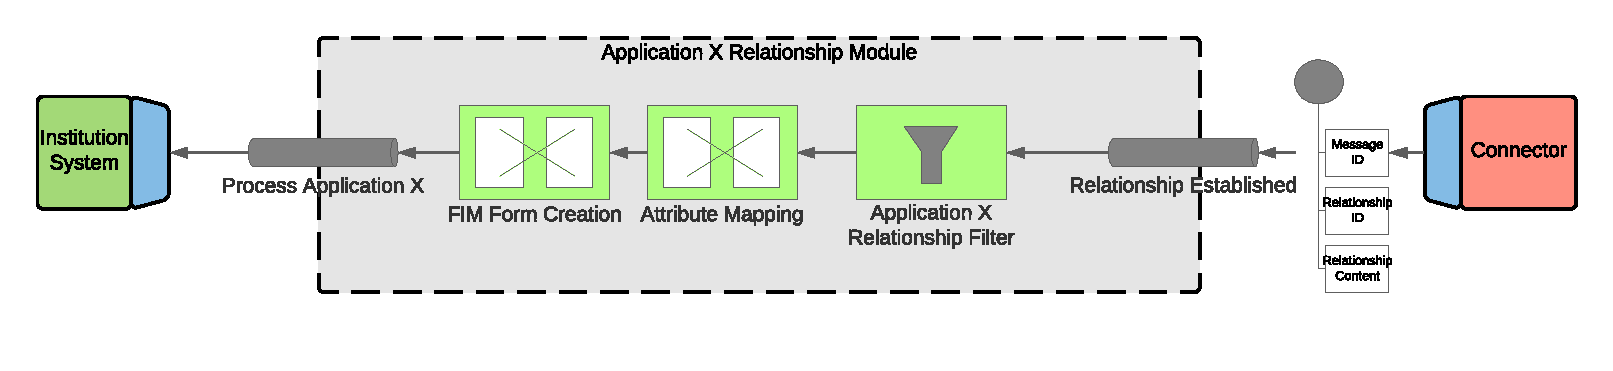
\includegraphics[scale=0.6]{Diagrams/Integration Architecture 2/Application Relationship Module.pdf}
\end{center}

Application Relationship Modules consume messages from the "Relationship Established" and filter all requests not concerning the application type of the module. After that, attributes shared as part of the relationship are mapped from the IMP data model to the OZG data model. As the existing institution system expects applications to be delivered as a form created by the form server of the administration portal, a message translator is added which translates the shared attributes to a suitable format so that the institution system understands it. The message is then published on the "Process Application" channel where a messaging adapter connected to the institution system consumes the message and submits the included form to the institution system the same way as the data exchange platform would.

The institution system can use the unique relationship ID as reference ID for the application process and all further user interactions.

Similar to the "Profile Attribute Change Message" module a "Application Attribute Change Message" module can be included witch performs the same operations.

\begin{center}
    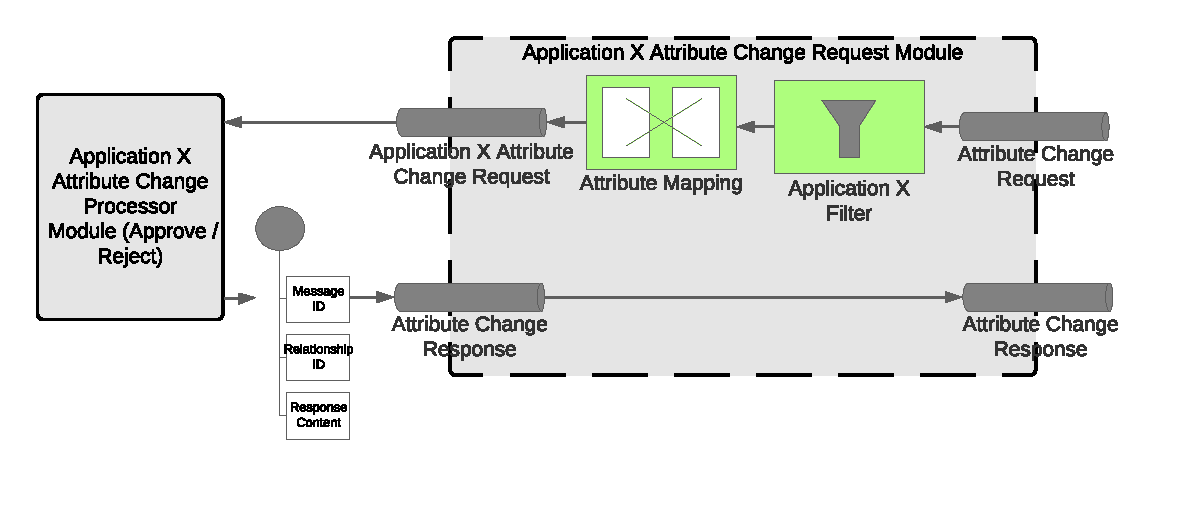
\includegraphics[scale=0.6]{Diagrams/Integration Architecture 2/Application Attribute Change Request Module.pdf}
\end{center}

For processing attribute change requests, application attribute change request modules are included for each relationship type. They consume messages from the !Attribute Change Request" channel and filter messages which do not concern the application type of the module. After mapping the attributes from IMP data model to OZG data model, messages are published on the "Application Attribute Change Request" channel. A module of the service provider can, based on the provided relationship ID and shared attributes decide if the attributes of the active application can still be changed. 

\begin{center}
    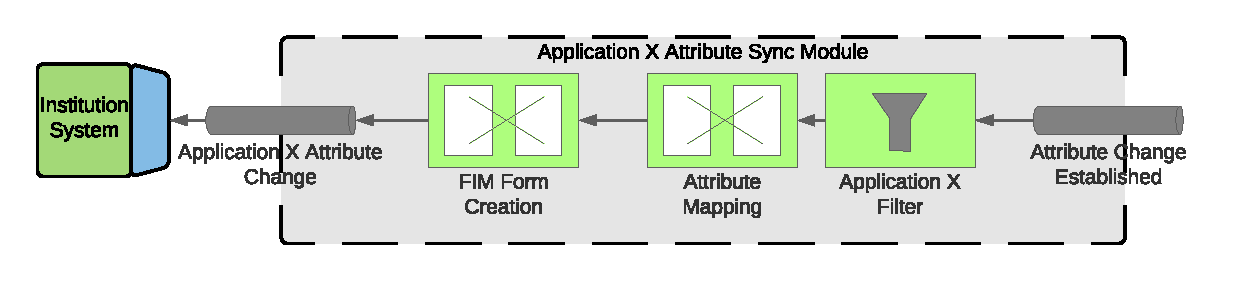
\includegraphics[scale=0.6]{Diagrams/Integration Architecture 2/Application Attribute Sync Module.pdf}
\end{center}

In order to process the change of an attribute for an active application, application attribute sync modules are included for each relationship type. They first filter all messages not concerning the relationship type of the module, then translate all attributes from the IMP data model to the OZG data model and publish them on the "Application Attribute Change" channel.
A messaging adapter connected to the service facade consumes the messages and submits it to the institution system. In case the institution system has no way of processing an attribute change, a message translator can be included which constructs a form the messaging adapter submits as a new application with the same relationship ID.

\begin{center}
    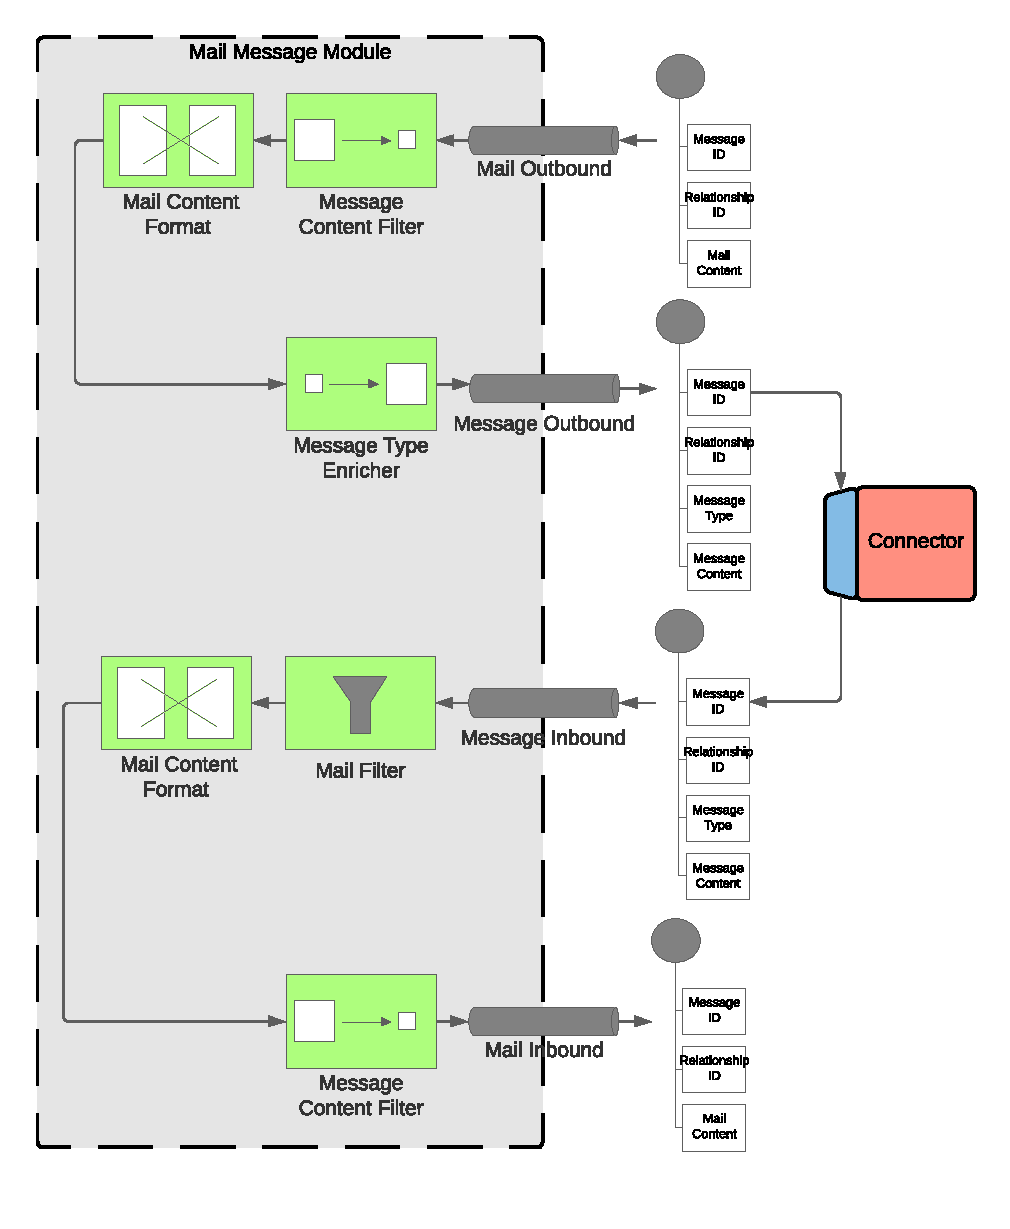
\includegraphics[scale=0.6]{Diagrams/Integration Architecture 2/Mail Message Module.pdf}
\end{center}

Using a bidirectional version of the "Mail Message" module, the messaging system can exchange mails from institution to IMP client and vice versa relating to a relationship ID.

\begin{center}
    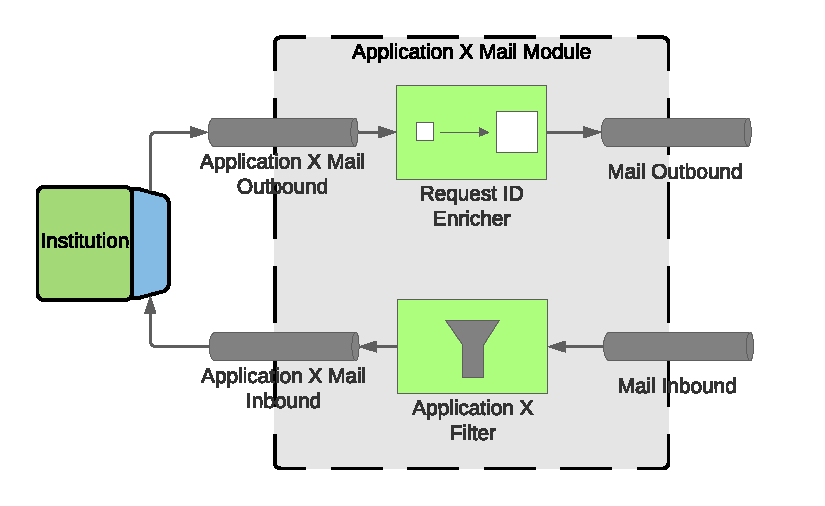
\includegraphics[scale=0.6]{Diagrams/Integration Architecture 2/Application Mail Module.pdf}
\end{center}

For exchanging mails, application mail modules are included for each type of application.